Temos uma fileira longa de copos e $n$ pedras no copo central (copo $0$).
Os seguintes movimentos são permitidos:

\textbf{Movimento tipo A}

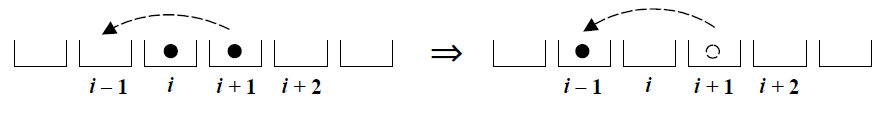
\includegraphics[width = 0.6\textwidth]{figuraA.png}

Se há pelo menos uma pedra no copo $i$ e pelo menos uma no copo $i + 1$ podemos fazer uma pedra que está no copo $i + 1$ pular para o copo $i - 1$ eliminando uma pedra do copo $i$.

\textbf{Movimento tipo B}

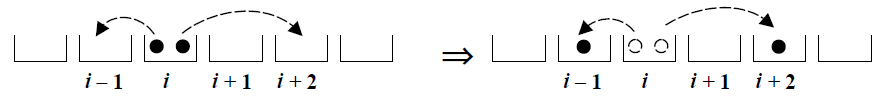
\includegraphics[width = 0.6\textwidth]{figuraB.png}

Se há pelo menos duas pedras no copo $i$ podemos pular uma para o copo $i + 2$ e uma outra para o copo $i - 1$.

Demonstre o seguinte fato: fazendo os movimentos tipo A ou B durante um tempo suficientemente longo sempre chegaremos a uma configuração a partir da qual não é mais possível fazer nenhum desses dois tipos de movimento.
Além disso essa configuração final não depende da escolha de movimentos durante o processo.